\Chapter{Project Implementation}

The GradeBadge application is designed to work on mobile devices and desktop computers. The UI of the application is developed using Bootstrap. When a page requires the data to be loaded from server or modified or deleted, a request is sent to the Web server over HTTP or HTTPS. The requests are sent to the Web server using Ajax. For handling Ajax requests and responses, this application uses JQuery Ajax API. All UI components are dynamically created or initialized in response to the data received from the Web server.

\newpage
\section{Welcome Screen}
When the GradeBoard application is loaded, a welcome screen with login button is presented to the user as shown in the Figure ~\ref{fig:welcome_screen}. The welcome screen shows application logo and login button for users to login to the system.

\vspace{3em}
\begin{figure}[H]
\begin{center}
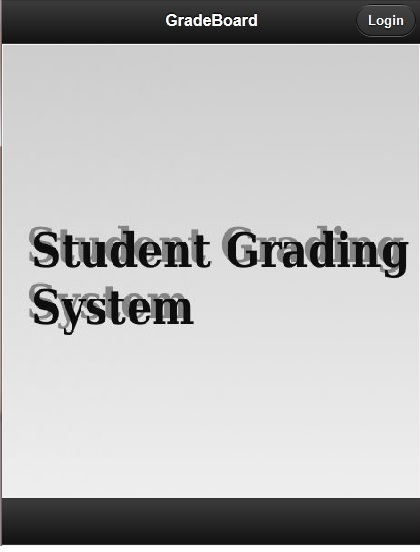
\includegraphics[height=3.8in,width=2.5in]{images/welcome_screen.jpg}
\caption{GradeBoard Welcome Screen}
\label{fig:welcome_screen}
\end{center}
\end{figure}

\newpage
\section{Login Screen}
GradBoard uses Google accounts for authentication and authorization. When the user clicks on the login button, the screen is automatically redirected to the Google login screen as shown in Figure~\ref{fig:login_screen}. There are two types of access users can get, namely admin and user. For admin access, the user is first authenticated by Google and then the user entry is checked in the admin table.  For user access, the user account is authenticated by Google. After logging in, the quarter screen is shown.

\vspace{3em}
\begin{figure}[H]
\begin{center}
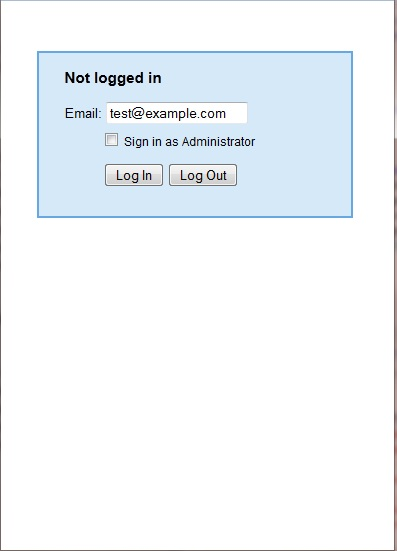
\includegraphics[height=3.8in,width=2.5in]{images/login_screen.jpg}
\caption{Login Screen}
\label{fig:login_screen}
\end{center}
\end{figure}

\newpage
\section{Quarter Screen}
The quarter screen displays quarter and year information as shown in Figure~\ref{fig:quarter_screen}. The quarter screen is shown after user logins into the system. After selecting quarter and year, the instructor clicks on the show courses button to view the list of courses.

\vspace{3em}
\begin{figure}[H]
\begin{center}
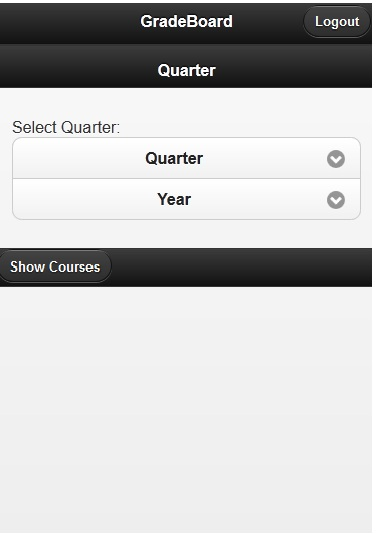
\includegraphics[height=3.8in,width=2.5in]{images/quarter_screen.jpg}
\caption{Quarter Screen}
\label{fig:quarter_screen}
\end{center}
\end{figure}

\newpage
\section{Courses Screen}
The courses screen shows a list of courses as shown in Figure~\ref{fig:courses_screen}. Using the courses screen, the instructor can add a new course or view the details of the existing course. After the user clicks on the course, the course details page is loaded.

\vspace{3em}
\begin{figure}[H]
\begin{center}
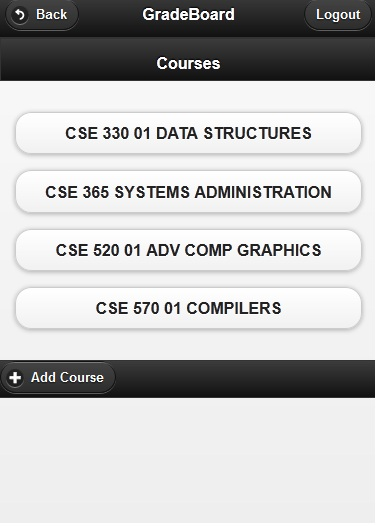
\includegraphics[height=3.8in,width=2.5in]{images/courses_screen.jpg}
\caption{Courses Screen}
\label{fig:courses_screen}
\end{center}
\end{figure}

\newpage
\section{Add Course Screen}
The add course screen is shown when the user clicks on the add button in the courses screen. Using this screen, instructors can add a new course as shown in Figure~\ref{fig:addcourse_screen}. This page checks that the course value entered already exists and displays an appropriate error message if not. The back button allows users to navigate to the course list page.

\vspace{3em}
\begin{figure}[H]
\begin{center}
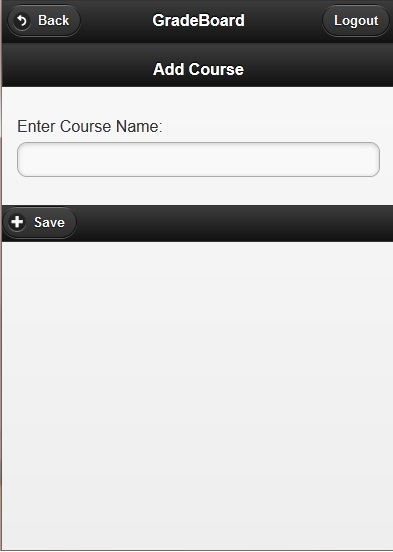
\includegraphics[height=3.8in,width=2.5in]{images/addcourse_screen.jpg}
\caption{Add Course Screen}
\label{fig:addcourse_screen}
\end{center}
\end{figure}

\newpage
\section{Course Details Screen}
The course details screen allows instructors to view course details such as the number of students registered and the number of seats available. The course details screen is shown in Figure~\ref{fig:coursedetails_screen}. From the course details screen, the user can edit the course, edit the grade components, or delete the course.

\vspace{3em}
\begin{figure}[H]
\begin{center}
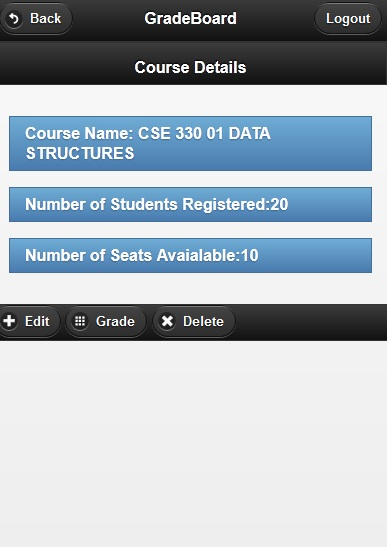
\includegraphics[height=3.8in,width=2.5in]{images/coursedetails_screen.jpg}
\caption{Course Details Screen}
\label{fig:coursedetails_screen}
\end{center}
\end{figure}

\newpage
\section{Edit Course Screen}
The edit course screen allows instructors to edit the course details as shown in Figure~\ref{fig:editcourse_screen}. The instructor can modify the course name, add additional instructors, add students and add gradable components.

\vspace{3em}
\begin{figure}[H]
\begin{center}
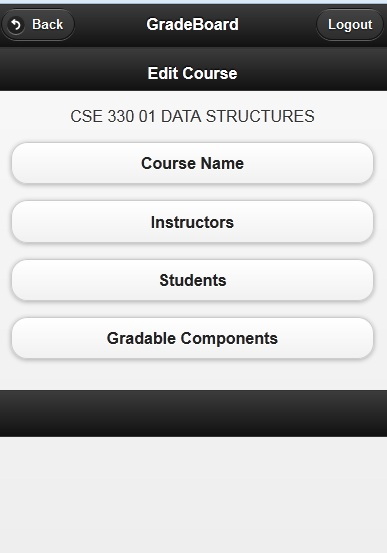
\includegraphics[height=3.8in,width=2.5in]{images/editcourse_screen.jpg}
\caption{Edit Course Screen}
\label{fig:editcourse_screen}
\end{center}
\end{figure}

\newpage
\section{Edit Course Name Screen}
The edit course name screen allows instructors to edit the course name as shown in Figure~\ref{fig:editcoursename_screen}. A validation is added to check if the course name entered by the user is empty or if it already exists. Changing the course name involves passing the current course name and new course name to the server. The server searches first the course entity with name equal to the current course name and then replaces the course name property value with the new course name.

\vspace{3em}
\begin{figure}[H]
\begin{center}
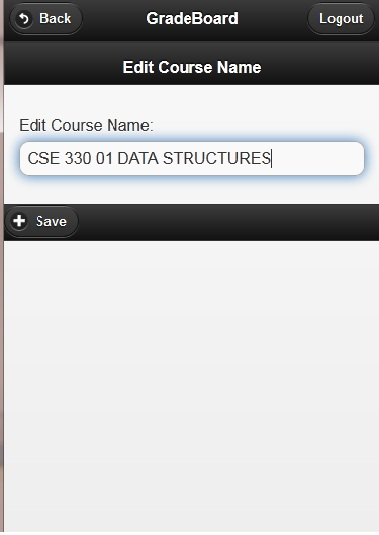
\includegraphics[height=3.8in,width=2.5in]{images/editcoursename_screen.jpg}
\caption{Edit Course Name Screen}
\label{fig:editcoursename_screen}
\end{center}
\end{figure}

\newpage
\section{Instructors Screen}
The instructors screen displays a list of instructors for a course as shown in Figure~\ref{fig:instructors_screen}. A course can have multiple instructors. Internally, instructors are stored as auth objects with a parent instructor (who created the course). Each auth object will contain the id of the course entity.

\vspace{3em}
\begin{figure}[H]
\begin{center}
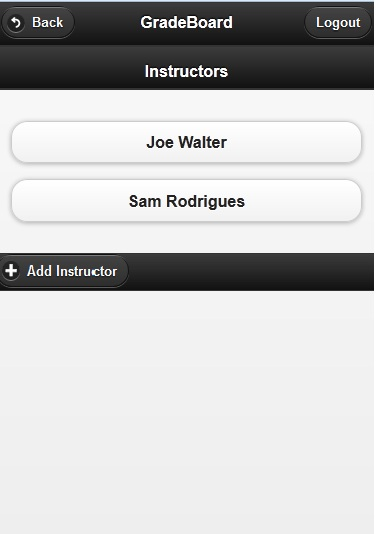
\includegraphics[height=3.8in,width=2.5in]{images/instructors_screen.jpg}
\caption{Instructors Screen}
\label{fig:instructors_screen}
\end{center}
\end{figure}

\newpage
\section{Add Insructor}
The add instructor screen allows an instructor to add another instructor as shown in Figure~\ref{fig:addinstructor_screen}. Only the instructor who originally created the course can add additional instructors. The new instructors have restricted access. Permission to change the course name or gradable components is not given to new instructors.

\vspace{3em}
\begin{figure}[H]
\begin{center}
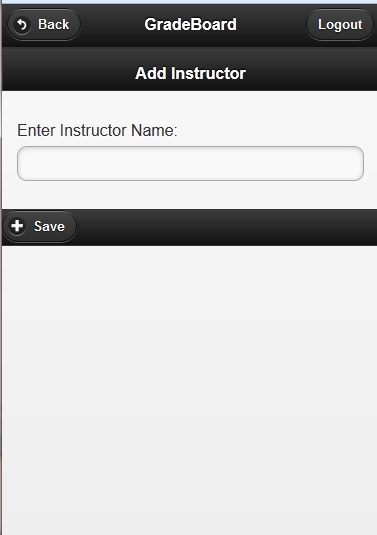
\includegraphics[height=3.8in,width=2.5in]{images/addinstructor_screen.jpg}
\caption{Add Instructor Screen}
\label{fig:addinstructor_screen}
\end{center}
\end{figure}

\newpage
\section{Delete Insructor}
The delete instructor screen allows the original instructor to remove an instructor from the course as shown in Figure~\ref{fig:deleteinstructor_screen}. The instructor who originally created the course can not be deleted, so there should always be at least one instructor for the course.

\vspace{3em}
\begin{figure}[H]
\begin{center}
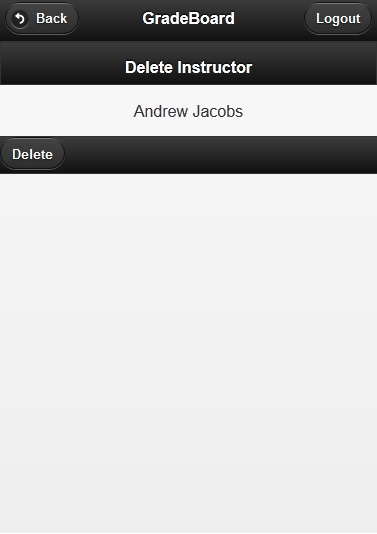
\includegraphics[height=3.8in,width=2.5in]{images/deleteinstructor_screen.jpg}
\caption{Delete Instructor Screen}
\label{fig:deleteinstructor_screen}
\end{center}
\end{figure}

\newpage
\section{Students}
The student screen lists all the students registered for the course as shown in Figure~\ref{fig:students_screen}. New students can be added by clicking on the add student button. There is also an option to add multiple students at once.

\vspace{3em}
\begin{figure}[H]
\begin{center}
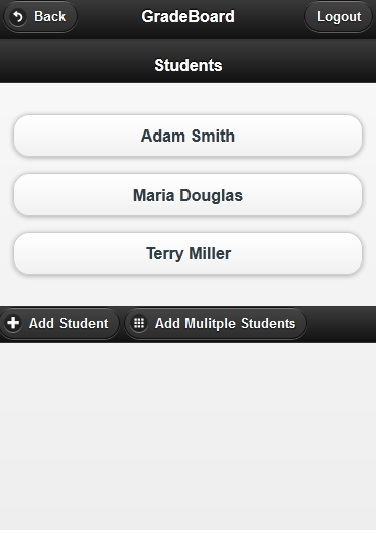
\includegraphics[height=3.8in,width=2.5in]{images/students_screen.jpg}
\caption{Students Screen}
\label{fig:students_screen}
\end{center}
\end{figure}

\newpage
\section{Add Student}
This screen allows instructors to add students to the course as shown in Figure~\ref{fig:addstudent_screen}. A validation is added to check for an empty student name or email address. Also, if a student with same name and email address already exists, an error message is shown to the instructor.
\vspace{3em}
\begin{figure}[H]
\begin{center}
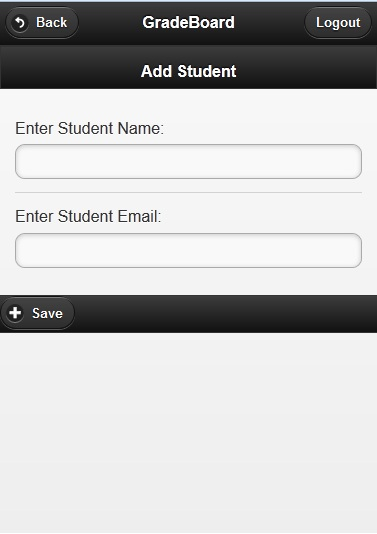
\includegraphics[height=3.8in,width=2.5in]{images/addstudent_screen.jpg}
\caption{Add Student Screen}
\label{fig:addstudent_screen}
\end{center}
\end{figure}

\newpage
\section{Add Multiple Students}
The add multiple students screen allows instructors to enter multiple student data at once as shown in Figure~\ref{fig:addstudentbulk_screen}. This helps the instructor to update student data at once when a course is created. To add multiple student data, instructors need to provide a comma separated list of student data in an HTML textarea field. The student data must contain three fields: first name, last name and email address. The instructor is notified if any student record is missing one of these fields.

\vspace{3em}
\begin{figure}[H]
\begin{center}
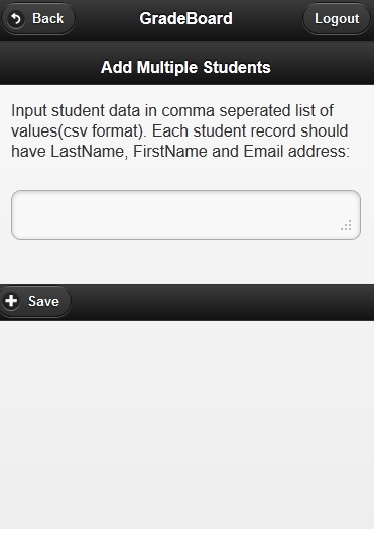
\includegraphics[height=3.8in,width=2.5in]{images/addstudentbulk_screen.jpg}
\caption{Add Multiple Students Screen}
\label{fig:addstudentbulk_screen}
\end{center}
\end{figure}


\newpage
\section{Edit Student}
The edit student screen allows instructors to edit the details of a student as shown in Figure~\ref{fig:editstudent_screen}. All of the student information can be changed by the instructor. 

\vspace{3em}
\begin{figure}[H]
\begin{center}
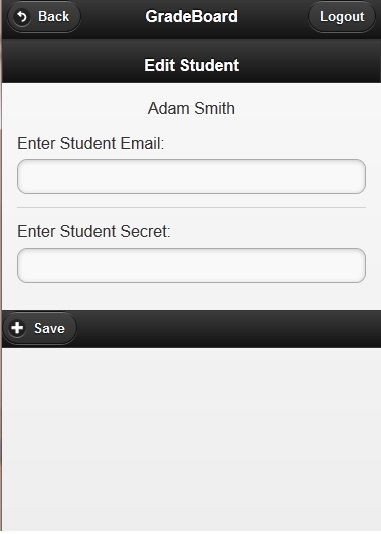
\includegraphics[height=3.8in,width=2.5in]{images/editstudent_screen.jpg}
\caption{Edit Student Screen}
\label{fig:editstudent_screen}
\end{center}
\end{figure}

\newpage
\section{Grades}
The grades screen shows an instructors list of the names of all gradable components as shown in Figure~\ref{fig:grades_screen}. If a new grade is required, then the instructor needs to add the gradable component in the add gradable component screen. Clicking on the grade button lists all the students registered for the course.

\vspace{3em}
\begin{figure}[H]
\begin{center}
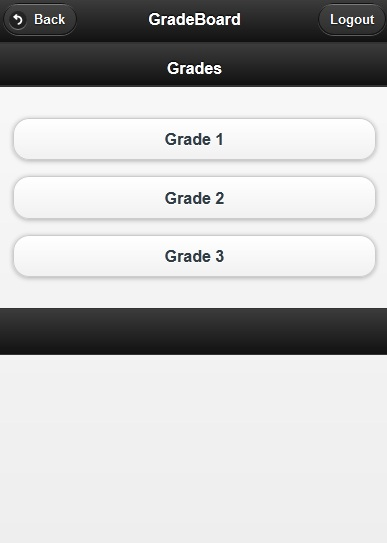
\includegraphics[height=3.8in,width=2.5in]{images/grades_screen.jpg}
\caption{Grades Screen}
\label{fig:grades_screen}
\end{center}
\end{figure}

\newpage
\section{Edit Grades}
The edit grade screen presents to the instructor a list of students whose grades can be edited as shown in Figure~\ref{fig:editgrades_screen}. Instructors can edit the individual grade by clicking on the student button. The view grade sheet option allows the instructor to view the grade sheet of the entire course.

\vspace{3em}
\begin{figure}[H]
\begin{center}
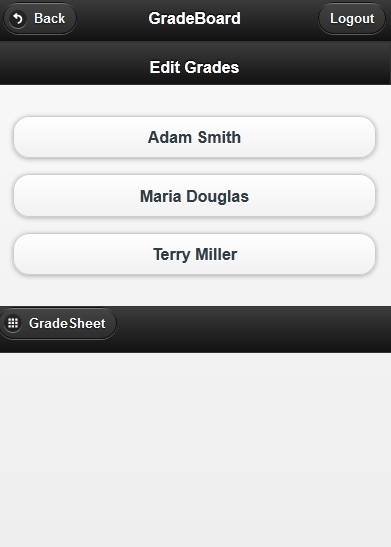
\includegraphics[height=3.8in,width=2.5in]{images/editgrades_screen.jpg}
\caption{Edit Grades Screen}
\label{fig:editgrades_screen}
\end{center}
\end{figure}

\newpage
\section{Edit Student Grade}
The edit student grade screen allows instructors to enter grade points of a student as shown in Figure~\ref{fig:editstudentgrade_screen}. A validation is provided to check that values are not empty and do not exceed the maximum value of grade points entered in the gradable component.

\vspace{3em}
\begin{figure}[H]
\begin{center}
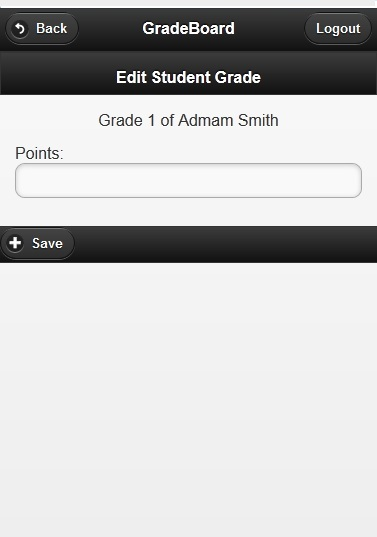
\includegraphics[height=3.8in,width=2.5in]{images/editstudentgrade_screen.jpg}
\caption{Edit Student Grade Screen}
\label{fig:editstudentgrade_screen}
\end{center}
\end{figure}


\newpage
\section{Gradable Components}
The gradable component screen displays a list of gradable components of a course as shown in Figure~\ref{fig:gradablecomponents_screen}. A new gradable component can be added by clicking on the add gradable component button.

\vspace{3em}
\begin{figure}[H]
\begin{center}
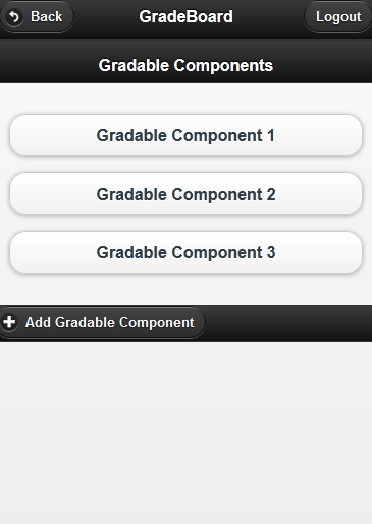
\includegraphics[height=3.8in,width=2.5in]{images/gradablecomponents_screen.jpg}
\caption{Gradable Component Screen}
\label{fig:gradablecomponents_screen}
\end{center}
\end{figure}

\newpage
\section{Add Gradable Component}
The add gradable component screen allows instructors to add a gradable component for the course as shown in Figure~\ref{fig:addgradablecomponent_screen}. Name, points and deadline are required fields and a validation is added to check for empty values. A check for duplicated entries is added to make sure gradable components are unique in a course.

\vspace{3em}
\begin{figure}[H]
\begin{center}
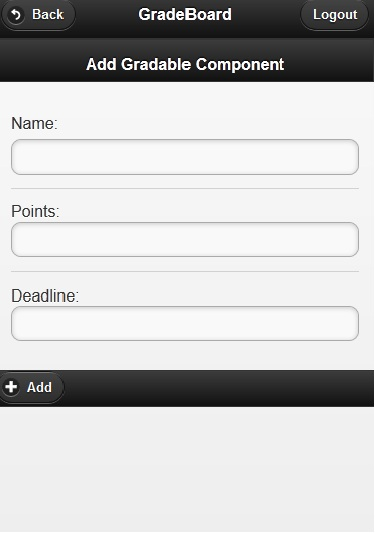
\includegraphics[height=3.8in,width=2.5in]{images/addgradablecomponent_screen.jpg}
\caption{Add Gradable Component Screen}
\label{fig:addgradablecomponent_screen}
\end{center}
\end{figure}

\newpage
\section{Edit Gradable Component}
The edit gradable component screen allows instructors to edit gradable components for the course as shown in Figure~\ref{fig:editgradablecomponent_screen}. Name, points and deadline are required fields, so a validation is performed to check for empty values.
\vspace{3em}
\begin{figure}[H]
\begin{center}
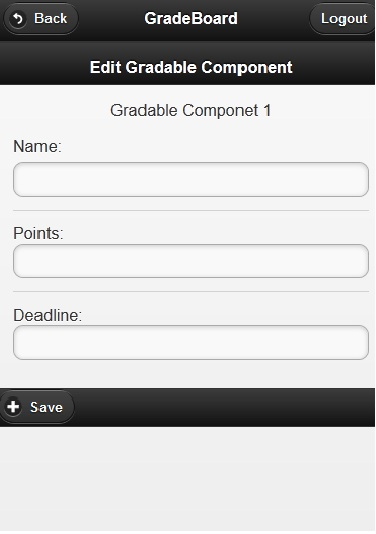
\includegraphics[height=3.8in,width=2.5in]{images/editgradablecomponent_screen.jpg}
\caption{Edit Gradable Component Screen}
\label{fig:editgradablecomponent_screen}
\end{center}
\end{figure}